\chapter{Results}

\section{Path to Police Station}
\begin{figure}[H]
    \centering
    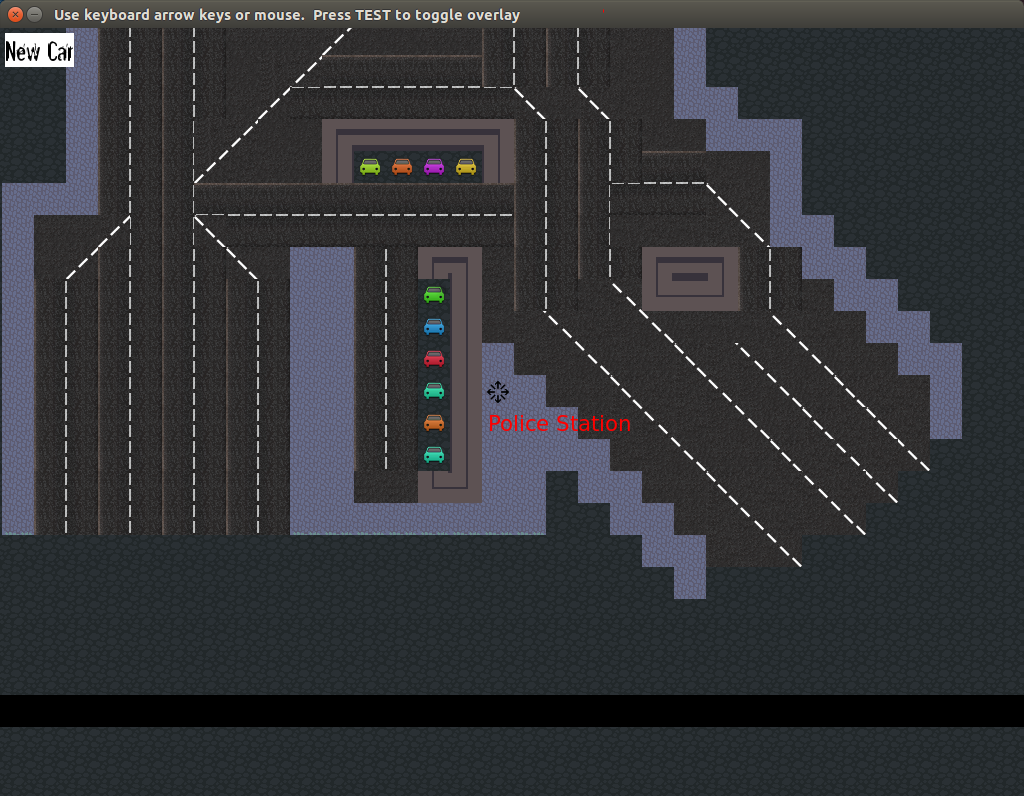
\includegraphics[width=1\textwidth]{images/path_to_police_station.png}
    \caption{Final ocuppied slots when requesting path to Police Station}
    \label{fig:path_to_police_station}
\end{figure}

\section{Path to Conferences Center}
Even though the g(x) distances were semi-randomly defined, it's finding the nearest slots that where defined in the configuration files.
\begin{figure}[H]
    \centering
    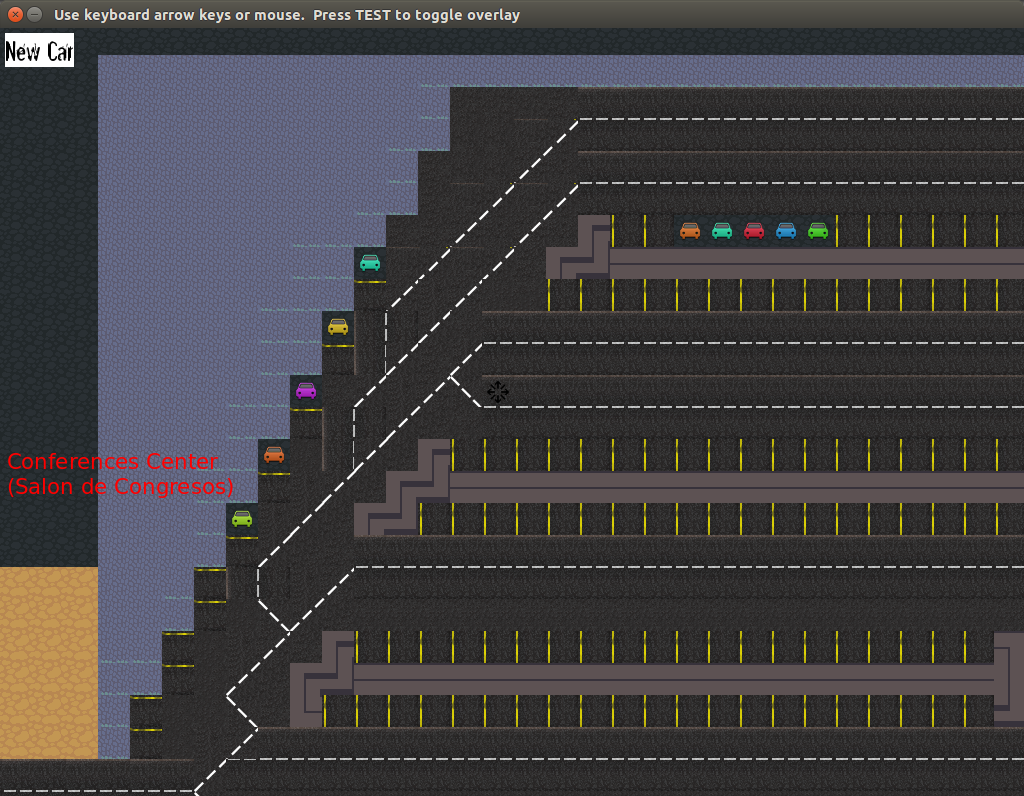
\includegraphics[width=.6\textwidth]{images/path_to_conferences_center.png}
    \caption{Final ocuppied slots when requesting path to Conferences Center}
    \label{fig:path_to_conferences_center}
\end{figure}
\section{Path to Residences}
When calculation path to Recidences, it took first the slots located in the second section (going from down-up) as the nearest 
area to the Recidences
\begin{figure}[H]
    \centering
    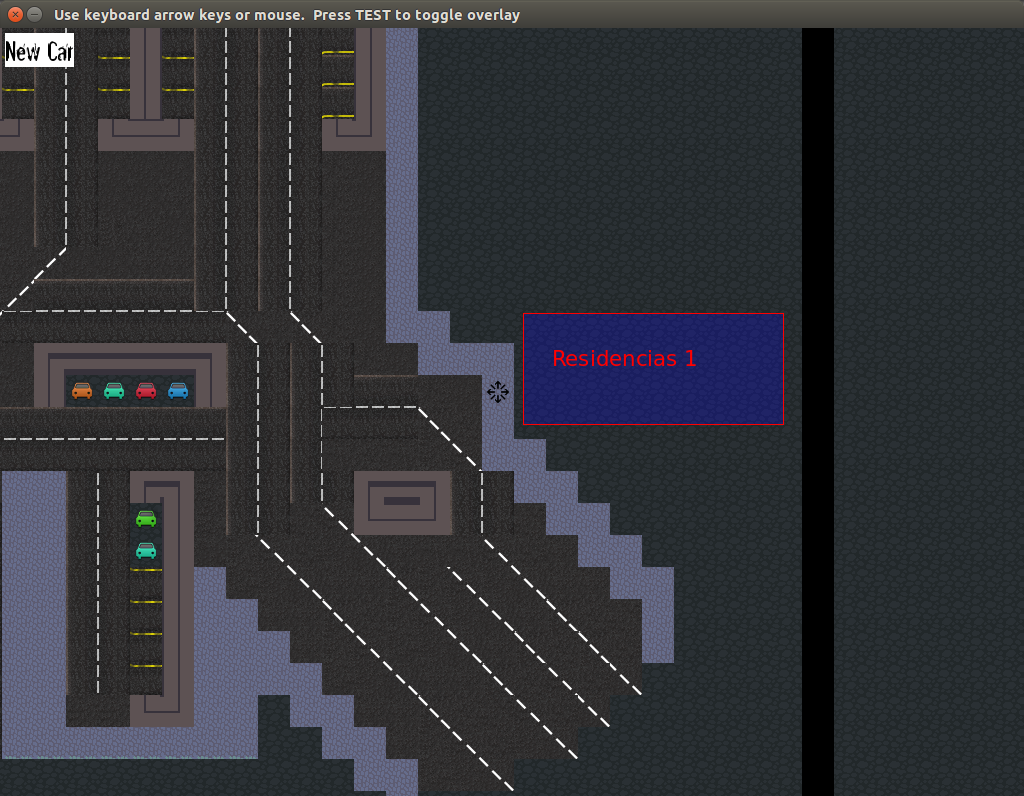
\includegraphics[width=.6\textwidth]{images/path_to_recidenses.png}
    \caption{Final ocuppied slots when requesting path to Recidenses}
    \label{fig:path_to_recidenses}
\end{figure}
